\chapter{Universal Malware Sample Encryption (UMSE)}

\section{Current malware sample shortcomings}

It is no surprise, it makes sense. Neither the end user nor the best antivirus
comparators\cite{AVComparatives2020}\cite{AVTest}, not even the most excellent and tested, have ever rated security
tools in this key aspect: confidentiality. The amount of client computer
leaked data by each accomplishes malware detection. When comparing them, they
only take into account some other factors currently much more in dispute. We
will refer to its table columns in the results: ``blocked'', ``user
dependent'', ``compromised'', ``protection rate'' and ``false
alarms''\cite{AVComparativesResults2019}.
  
\begin{figure}[h]
  \centering
  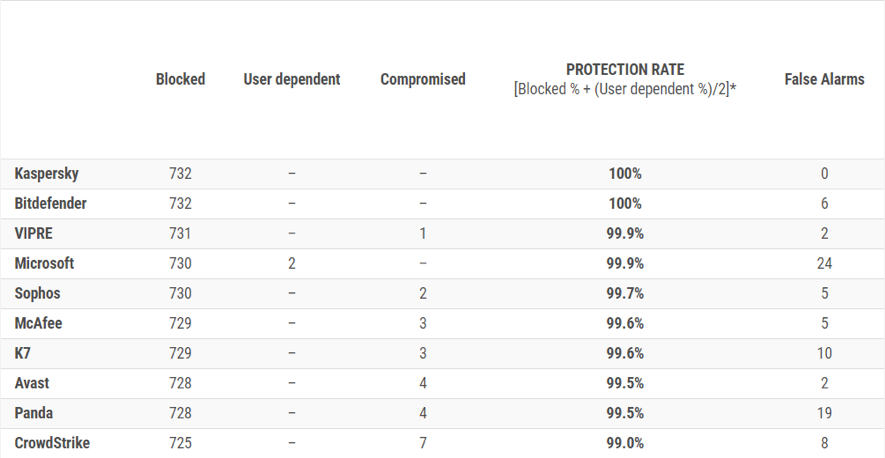
\includegraphics[width=0.99\textwidth]{./figures/MalwareSample}
\end{figure}

Therefore, all antiviruses are good in detection and this explains different
results drawn months apart when comparing them but, how good are they in
confidentiality? Just note how important confidentiality is for the user when
choosing between antimalware products.

Taking up the issue of what malware sample currently is, we should add that,
sometimes, in order to mitigate risks in transport, storage and sample
sharing, this functional file is wrapped in a compression format like PKZIP
and, when supported by such format, maybe encrypted also by the de facto key,
i.e., the symmetric but publicly known key:
``infected''\cite{ZeltserShareMalware}\cite{VXVault2020}\cite{VirusTotalFileSearch2020}\cite{MalShare2020}\cite{VirusShare2020}\cite{VirusBay2020} The following picture shows a
threat intelligence website in which files are downloaded in this way but the
reader should know \texttt{Malwarebytes} uses this mechanisms because it was
analyzed and shown in section~\ref{sec:}
\begin{figure}[h]
  \centering
  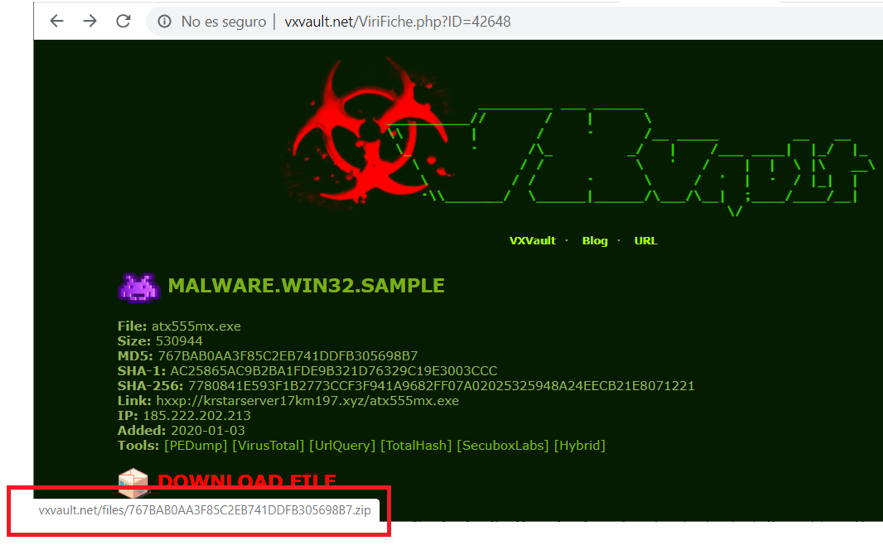
\includegraphics[width=0.99\textwidth]{./figures/ThreatWebsite}
\end{figure}

This way of acquiring and storing malware samples, as is evident, was
improvised but not seriously thought. In summary, the approach has the
following shortcomings:
\begin{enumerate}
\item Identification shortcoming: Given a malware sample, it is not possible
  to know, a priori, if the file is a malware sample or not. It is, at every
  respect, simply a compressed file.

\item Universality shortcoming: A malware sample is not a file. Malware,
  according to UMSE, is an element or a set of elements, hardware, software
  and/or firmware which framed in a context and in a state of its life cycle
  is determinated malicious. Accordingly, a malware element can be
  ``fileless'' or, in a given moment of its life cycle, to be volatile,
  located only in principal memory (like it happens with
  \texttt{DoublePulsar}, to name an example) and this must not be a problem
  when taking a malware sample. To put it differently, the sample must contain
  the element or the set of elements indicating its nature and all of those
  metainformation which is considered necessary.
  
\item Contextualization shortcoming: Context is lost. The sample is usually is
  a file without context. This lost will take unfortunate consequences in
  subsequent phases of the reverse engineering process.

\item Standardization shortcoming: The analyst does not know what kind of
  element is dealing with when he/she gets a sample, or how it came to be a
  sample. A real life example: During compression and decompression processes,
  it usually happens that, for instance, the compression format, being
  arbitrary, does not allow to store all file attributes and enters spurious
  values when decompressed.

\item Confidentiality shortcoming: Potentially confidential data stored in the
  samples is not protected in any way. Therefore, this data will be revealed
  to analysts, companies and intelligence organizations and/or partners or
  whoever malware sample is shared with. This data far exceeds the ``need to
  know'' principle, that is, the amount of information the professional really
  needs in order to do his/her job. We can put an easy-to-understand example
  of this risk. If an office file has aroused malware suspicion and it has
  macros, it is common sense to examine the macros at first and, if the code
  in macros code is not sufficient then, using the concept of encrypted
  malware sample proposed in this work, to decrypt other parts of the file
  content usually more confidential and less malware-prone but keeping a log
  of this decryption operations.
  
\item Authentication shortcoming: It is not possible to determine the
  authenticity of a sample if it was modified after acquisition. Note that
  authentication is also necessary to support encryption in order to guarantee
  confidentiality.
\end{enumerate}

\section{Universal Malware Sample Encryprtion}

\textbf{Universal Malware Sample Encryption format}, (henceforth, UMSE), is a
specific universal file format for malware samples, making efforts in
efficient acquisition, transport and storage which preserves confidentiality,
authenticity and makes possible the potential samples sensitive data access
registration.

\subsection{UMSE universality}

This format is declared to be \textbf{universal} because it supports the
storage of any kind of potential malware sample (contextualized and metadata
enriched) covering any possible state of its life cycle. Expanding, therefore,
the current malware sample concept\cite{ZeltserShareMalware} (limited to files) to a more general
concept which allows the right storage of any element software, hardware
and/or firmware.  Understanding by elements software, hardware and/or
firmware: system processes, program parameters, environment variables,
register entries, network traffic captures, memory content, file paths and
other file system information, integrated circuits photos and schemes, etc.

\subsection{UMSE as a sample format}

As UMSE is a format purposely designed for malware samples, \textbf{any file
  given in such format can be identified as malware sample}. Those malware
samples can be easily identified by its magic ASCII value located at the very
beginning of the file: “UMSE”. It is also specifically \textbf{stored in a
  standard format, minimizing the loss of sample context information by itself
  and its parts. While keeping the maximum storage and sharing security}.

\subsection{UMSE confidentiality}

UMSE format allows also to preserve potentially sensible data in the samples
by confidentiality. This is achieved through a symmetric cipher. Symmetric
keys are randomly generated (and IVs are also randomly generated) and wrapped
with a public RSA key.  Each symmetric key is associated to a confidentiality
level. Each sample is divided in parts and each part is evaluated to assign a
confidentiality level to it. Therefore, only a sufficiently privileged analyst
will be able to decrypt a sample part and, every time a key is revealed to him
by RSA private key decryption, the event could be registered.

\subsection{UMSE authentication}

Each sample is HMAC authenticated following an Encrypt-then-MAC (EtM)
scheme\cite{AuthenticatedEncryption2000}. HMAC key is derived from the symmetric keys sequential list,
initialization vectors and associated confidentiality levels. Therefore, only
people who knows all the symmetric keys and initialization vectors (this fact
means knowing the entire decrypted sample) could be able to modify it. This
protects the sample from ``downgrade'' attacks to the confidentiality level of
its parts, from ``decryption oracle attacks'', etc.

\section{UMSE format specification}

\subsection{Formal specification}

UMSE structure is formally specified using Kaitai Struct language\cite{KaitaiStructDoc}.

\begin{tcolorbox}
  \small
\begin{verbatim}
 1 meta:
 2   id: umse
 3   file-extension: umse
 4   endian: le
 5 
 6 seq:
 7   - id: umse_header
 8     type: header 
 9   - id: decryption_table
10     type: decryption_table
11     repeat: expr 
12     repeat-expr: umse_header.num_records_dec_table
13   - id: entry
14     type: entry
15     repeat: expr 
16     repeat-expr: umse_header.num_file_entries
17   - id: file_properties
18     type: file_properties
19   - id: authentication_header
20     type: authentication_header
21 
22 types:
23   header:
24     seq:
25       - id: magic
26         contents: UMSE
27         doc: "Magic of: Universal Malware Sample Encryption" 
28       - id: version
29         type: str
30         encoding: UTF-8
31         size: 4
32         doc: "Magic of: Universal Malware Sample Encryption"
33       - id: num_records_dec_table
34         type: u4 
35         doc: "Number of Records in Decryption Table"
36       - id: num_file_entries
37         type: u4 
38         doc: "Number of file entries or encrypted byte chunks"
39       - id: author_name_length
40         type: u4 
41         doc: "Author name length"
\end{verbatim}
\end{tcolorbox}

\begin{tcolorbox}
  \small
\begin{verbatim}
42       - id: author_name
43         type: str
44         size: author_name_length
45         encoding: UTF-8
46         doc: "Author name"
47   decryption_table:
48     seq:
49       - id: level_of_confidentiality
50         type: u1 
51       - id: aes_wrapped
52         type: u1 
53         repeat: expr
54         repeat-expr: 256
55   entry:
56     seq:
57       - id: size 
58         type: u4 
59       - id: level_of_confidentiality
60         type: u1 
61       - id: encrypted_message
62         type: u1 
63         repeat: expr
64         repeat-expr: size
65       - id: num_metadata
66         type: u4 
67       - id: entry_metadata
68         type: entry_metadata 
69         repeat: expr
70         repeat-expr: num_metadata
71         if: num_metadata > 0
72   entry_metadata:
73     seq:
74       - id: tag
75         type: u1 
76         repeat: expr
77         repeat-expr: 8
78       - id: length
79         type: u4 
80       - id: value
81         type: u1 
82         repeat: expr
83         repeat-expr: length
\end{verbatim}
\end{tcolorbox}

\begin{tcolorbox}
  \small
\begin{verbatim}
84   file_properties:
85     seq:
86       - id: level_of_confidentiality
87         type: u1
88       - id: hash_value
89         type: u1 
90         repeat: expr
91         repeat-expr: 32
92       - id: num_metadata
93         type: u4 
94       - id: file_metadata
95         type: file_metadata 
96         repeat: expr
97         repeat-expr: num_metadata
98         if: num_metadata > 0
99   file_metadata: 
100    seq:
101       - id: tag
102         type: u1 
103         repeat: expr
104         repeat-expr: 8
105       - id: length
106         type: u4 
107       - id: value
108         type: u1 
109         repeat: expr
110         repeat-expr: length
111   authentication_header:
112     seq:
113       - id: length
114         type: u4 
115         doc: "HMAC length"
116       - id: hmac 
117         type: u1 
118         repeat: expr
119         repeat-expr: length
120         doc: "HMAC"
121  rsa_private_key:
122    seq:
123      - id: length
124        type: u4
125        if: not _io.eof
126        doc: "RSA private key length"
127      - id: rsa_private_key
128        type: u1
129        repeat: expr
130        repeat-expr: length
131        if: not _io.eof
142        doc: "RSA private key"
\end{verbatim}
\end{tcolorbox}

For practical purposes, an UMSE format structure parser template was also
developed:

\begin{tcolorbox}
  \footnotesize
\begin{verbatim}
 1  //------------------------------------------------
 2  //--- 010 Editor v8.0.1 Binary Template
 3  //
 4  //      File: umse.bt
 5  //   Authors: David Alvarez Perez
 6  //   Version: 0.1
 7  //   Purpose: Template for Universal Malware Sample Encryption
 8  //  Category: Misc
 9  // File Mask: umse
10  //  ID Bytes: 55 4D 53 45 //UMSE
11  //   History: 
12  //------------------------------------------------
13
14  struct ENCRYPTED_SAMPLE {
15     struct HEADER
16         char    magic[4] <comment="Magic of: Universal Malware Sample 
                                      Encryption">;
17         char    version[4] <comment="Version of: Universal Malware 
                                        Sample Encryption format">;
18         int     numRecordsDecTable <comment="Number of Records in 
                                                Decryption Table">;
19         int     numFileEntries <comment="Number of file entries or 
                                            encrypted byte chunks">;
20         int     authorNameLength <comment="Author name length">;
21         char    authorNameValue[header.authorNameLength] 
                                    <comment="Author name">;
22      header;	
23 
24     struct DECRYPTION_TABLE 
25         char    levelOfConfidentiality <comment="Level of 
                                                    confidentiality">;
26         char    aesWrapped[256] <comment="IV and AES256 Key 
                                            (wrapped with Public RSA) both 
                                            necessaries to decrypt chunks 
                                            of this level">;
27      decryptionTable [ header.numRecordsDecTable ];
28 
\end{verbatim}
\end{tcolorbox}

\begin{tcolorbox}
  \footnotesize
\begin{verbatim}
29     struct ENTRY 
30         int     size <comment="Size of this entry">;
31         char    levelOfConfidentiality <comment="Level of 
                                            confidentiality of this entry">;
32         char    encryptedMessage[entry.size] <comment="Encrypted chunk">;
33         int     numMetadata <comment="Number of public metadata entries 
                                         of this chunk">;
34         struct ENTRY_METADATA 
35             char    tag[8] <comment="TAG of this metadata">;
36             int     length <comment="Size of this metadata content">;
37             char    value[ length ] <comment="metadata value">;
38          entry_meta [ entry. numMetadata ]<optimize=false>;
39      entry [ header.numFileEntries ]<optimize=false>;
40 
41     struct FILE_PROPERTIES 
42         char    levelOfConfidentiality <comment="File confidentiality level">;
43         char    hashValue[ 32 ] <comment="Hash value">;
44         int     numMetadata <comment=" Number of public metadata entries 
                                          of this file">;
45         struct FILE_METADATA 
46             char    tag[8] <comment="TAG of this flag">;
47             int     length <comment="Size of this metadata content">;
48             char    value[ file_metadata.length ] <comment="metadata value">;
49          file_metadata [ file_properties.numMetadata ]<optimize=false>;
50      file_properties;
51 
52     struct AUTHENTICATION_HEADER 
53         int     authenticationLength  <comment="Authentication length">;
54         char    authentication[authentication_header.authenticationLength]  
             <comment="HMAC SHA256 Authentication. The key is the sha256 of 
                       the encryption table but after entire decrypted">;
55      authentication_header; 
56
57     if(!FEof()) {
58         struct RSA_PRIVATE_KEY {
59             int     rsaPrivateKeyLength <comment=" RSA Key Length">;
60             char    rsaPrivateKey[ rsa_private_key.rsaPrivateKeyLength ] 
                  <comment="RSA Key">;
61         } rsa_private_key <comment="RSA Key (This is an optional field)">;
62     }
63  } encryptedSample; 
64
\end{verbatim}
\end{tcolorbox}
\begin{tcolorbox}
  \small
\begin{verbatim}
65
66  // Main
67
68  int isUMSE(void)
69  {
70      local TFindResults countUmse;
71      countUmse = FindAll("UMSE");
72      return countUmse.count;
73  }
74
75
76  isUMSE();
77  if (isUMSE()==0)
78  {
79      Printf("Keywords not found, not a UMSE file!\n");
80      return;
81  }
\end{verbatim}
\end{tcolorbox}

\subsection{Overview}

A sample given in UMSE format consists in the following sub-structures:
\begin{itemize}
\item UMSE header.
\item Decryption table.
\item Entries.
\item File properties.
\item Authentication header.
\item RSA Private key (this is an optional field).
\end{itemize}

In the following picture an example of UMSE file format structure is shown.
\begin{figure}[h]
  \centering
  \includegraphics[width=0.5\textwidth]{./figures/UMSEFormat}
\end{figure}

\subsection{UMSE header}
As you can appreciate, this format is first formed by a \texttt{HEADER} header
consisting of the following fields:
\begin{itemize}
\item The \texttt{Magic} field. Whose value is always \texttt{UMSE}. This value
  allows to easily identify that it is an UMSE format file.
\item The \texttt{Version} field. A string of four characters indicating UMSE
  version. The current version string is: \texttt{1.0}.
\item The \texttt{numRecordsDecTable} field. This field indicates, by using an
  integer of 4 bytes, the number of entries of which \texttt{Decryption Table}
  is composed, I mean, the number of AES keys stored in the UMSE file (an AES
  key for each possible confidentiality level).
\item The \texttt{numFileEntries} field. This field indicates, by using an
  integer of 4 bytes, the number of chunks stored in the UMSE sample.
\item The \texttt{authorNameLength} field indicates, by using an integer of 4
  bytes, the size of the next field (\texttt{authorNameValue}).
\item The field \texttt{authorNameValue} the name of the malware samples
  author.
\end{itemize}
\begin{figure}[h]
  \centering
  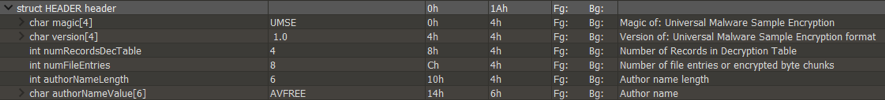
\includegraphics[width=0.99\textwidth]{./figures/UMSEHeader}
\end{figure}

\subsection{Decryption table}

Next, there is the \texttt{Decryption table}. This table contains AES
keys and IVs asociated to each confidentiality level. This keys are used to
encrypt chunks regarding the confidentiality level.  Each table entry contains
an AES key and IV, both wrapped with RSA public key and stored into the
\texttt{aesWrapped} field. And corresponding confidentiality level is stored
into \texttt{levelOfConfidentiality} field.
\begin{figure}[h]
  \centering
  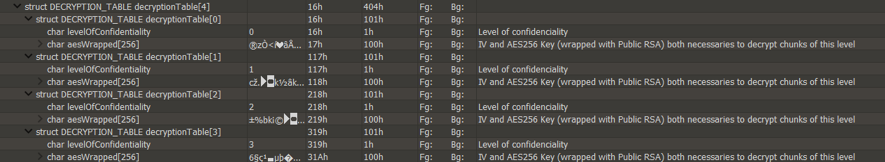
\includegraphics[width=0.99\textwidth]{./figures/UMSEDT}
\end{figure}

\subsection{Entries}

Each sample chunk is stored (encrypted) as an entry regarding its
confidentiality level. Each entry has: a field named \texttt{size} indicating
the size of the encrypted content, a field named
\texttt{levelOfConfidentiality} indicating the chunk encrypted confidentiality
level, a field named \texttt{encryptedMessage} containing the encrypted chunk,
a field named \texttt{numMetadata} indicating the number of metadata entries
associated to the chunk.
\begin{figure}[h]
  \centering
  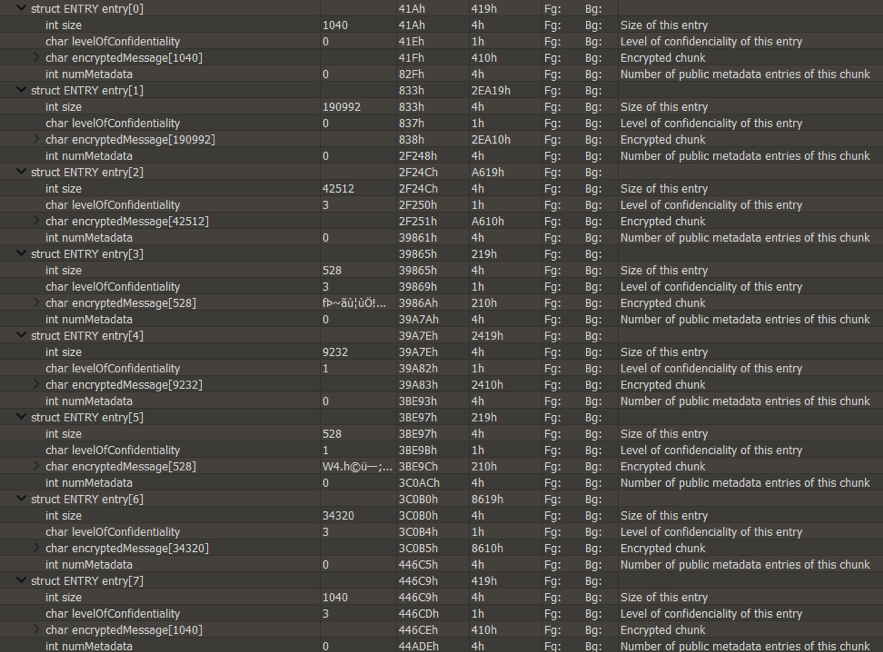
\includegraphics[width=0.99\textwidth]{./figures/UMSEEntries}
\end{figure}

\subsection{File properties}
An additional entry indicating properties which applies to the entire file do
exist.
\begin{figure}[h]
  \centering
  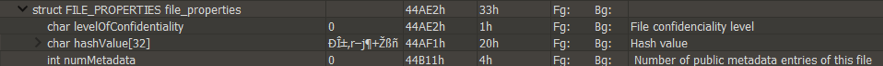
\includegraphics[width=0.99\textwidth]{./figures/UMSEFP}
\end{figure}

\subsection{Authentication header}

Finally, an HMAC checksum of the file is generated. The key used to generate
this HMAC checksum is the SHA256 hash of the RSA decrypted \texttt{decryption
  table}.
\begin{figure}[h]
  \centering
  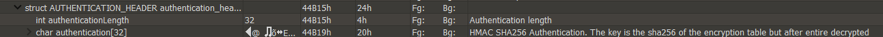
\includegraphics[width=0.99\textwidth]{./figures/UMSEAH}
\end{figure}

Authentication header is absolutely necessary. For instance, an analyst who
has not sufficient privilege to decrypt an UMSE entry, will not be able to
generate another UMSE file with the entry confidentiality level downgraded, in
order to decrypt it.  It protects from padding oracle attacks\cite{Eurocrypt2002}\cite{Oaep} as well. This
block is complementary to encryption.

\subsection{RSA private key}

This is an optional (and generally not recommended) field used to embed the
private RSA key into the file. It can be useful in some cases when
confidentiality is not an issue but the analyst want to exploit the UMSE
format capabilities (see section: 12.5 UMSE tools).
\begin{figure}[h]
  \centering
  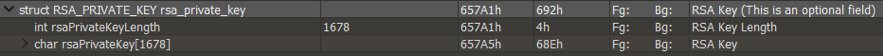
\includegraphics[width=0.99\textwidth]{./figures/UMSEPK}
\end{figure}

\section{UMSE implementation}

\subsection{UMSE C/C++ library}
A C/C++ library was developed to work more easily with UMSE. As most of
security products are developed in C/C++, the UMSE library was developed in
these languages but note that it can be used with independence of the
programming language, for instance, the author integrated it with Python and,
obviously, it worked. The library project follows a standard C project
structure\cite{CanonicalProjectStructure} (see Figure~\ref{fig:UMSELibrary}:
\begin{itemize}
\item \texttt{bin} directory: Compiled resulting binaries are putted inside
  this directory.
\item \texttt{build}: Building files are putted in this directory.
\item \texttt{doc} Documentation directory.
\item \texttt{include}: Includes are here. A subfolder named \texttt{include}
  also exists and it is used to store third party includes.
\item \texttt{lib}: Library files are stored here.
\item \texttt{src}: The program source code.
\item \texttt{test}: Some code to test the library.
\end{itemize}

\begin{figure}
  \centering
  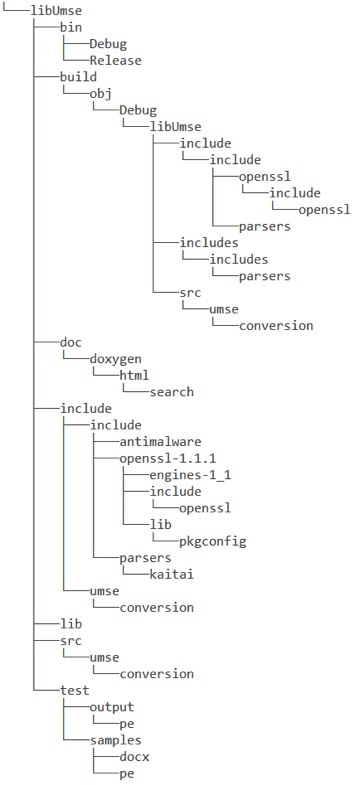
\includegraphics[width=0.5\textwidth]{./figures/UMSELibrary}
  \caption{\label{fig:UMSELibrary} Structure of the UMSE library.}
\end{figure}
\begin{figure}
  \centering
  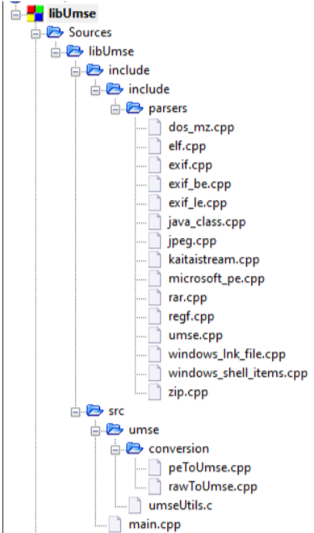
\includegraphics[width=0.5\textwidth]{./figures/UMSEProject}
  \caption{\label{fig:UMSELibrary} Organization of the UMSE project.}
\end{figure}

The project content can be summarized as follows
(Figure~\ref{fig:UMSEProject}):
\begin{itemize}
\item the \texttt{parsers} directory contains a lot of common file type
  parsers for C++. These parsers were generated automatically by Kaitai
  Struct. Parsers folder includes also \texttt{umse.cpp} in order to
  demonstrate that UMSE specification works as expected and it is implemented.
\item the \texttt{conversion} directory implements the conversion from every
  specific file format or chunk structure to UMSE. In file headers of each
  file format/chunk structure converter are defined parameters to calculate
  the corresponding confidentiality level of each file part.
\item the \texttt{umseUtils.c} all necessary functions to deal with UMSE file
  format are developed here. It is not dependent from Kaitai Struct in order
  to allow you to re-use it in other projects.
\item the \texttt{main.cpp} library exported functions are written here and
  some testing/debugging code is also written here.
\end{itemize}

The library exported functions are displayed in
Tables~\ref{fig:f1}-\ref{fig:f3}.
\begin{table}
  \centering
  \begin{tabular}{|l|p{0.7\textwidth}|} \hline
    Description	& This function converts a chunk to Universal Malware Sample
                  Encryption format. \\ \hline
    Input parameters &	\texttt{chunkLength} \\
                     & \texttt{chunk} \\ \hline
    Output parameters & \texttt{umseSize} \\
                      & \texttt{umse} \\ \hline
    Return value & \texttt{void} \\ \hline
    Function header	&
\begin{verbatim}
void DLL_EXPORT ChunkToUmse(
        unsigned int chunkLength,
        unsigned char* chunk,
        unsigned int* umseSize,
        unsigned char** umse
);
\end{verbatim}
    \\ \hline
  \end{tabular}
  \caption{\label{fig:f1} Function f1.}
\end{table}
\begin{table}
  \centering
  \begin{tabular}{|l|p{0.7\textwidth}|} \hline
    Description	& If UMSE integrity check is successful, this function
                  decrypts an entry of a given Universal Malware Sample
                  Encryption file chunk and its RSA Private key.  \\ \hline
    Input parameters &	\texttt{chunkLength} \\
                & \texttt{chunk} \\
                & \texttt{entryToDecrypt} \\
                & \texttt{accessLevel} \\
                & \texttt{rsaPrivateKey} \\ \hline
    Output parameters & \texttt{decryptedEntryLength} \\
                      & \texttt{decryptedEntry} \\ \hline
    Return value & $-2$ if integrity check iss not successful \\
                & $-1$ if \texttt{entryToDecrypt} does not exist \\
    & $0$ if the function ends without errors. \\ \hline
    Function header	&
\begin{verbatim}
int DLL_EXPORT DecryptUmse(
        unsigned int umseLength,
        unsigned char* umse,
        unsigned int entryToDecrypt,
        unsigned int accessLevel,
        char* rsaPrivateKey,
        unsigned int* decryptedEntryLength,
        unsigned char** decryptedEntry
);
\end{verbatim}
    \\ \hline
  \end{tabular}
  \caption{\label{fig:f2} Function f2.}
\end{table}
\begin{table}
  \centering
  \begin{tabular}{|l|p{0.7\textwidth}|} \hline
    Description	& This function checks UMSE integrity.  \\ \hline
    Input parameters &	\texttt{chunkLength} \\
                & \texttt{chunkLength unsigned int} \\
                & \texttt{chunk unsigned char *} \\ \hline
    Output parameters & \texttt{umseSize unsigned int *} \\
                      & \texttt{umse unsigned char **} \\ \hline
    Return value & True if integrity check is successful, otherwise it returns
    false \\ \hline
    Function header	&
\begin{verbatim}
bool DLL_EXPORT CheckUmseIntegrity(
                unsigned int umseLength,
                unsigned char* umse,
                char* rsaPrivateKey
);
\end{verbatim}
    \\ \hline
  \end{tabular}
  \caption{\label{fig:f3} Function f3.}
\end{table}

\section{UMSE agent}

The UMSE Agent is an extremely simple Python program to demonstrate how to
collect system elements, transform it to UMSE, and sent the resulting UMSE
samples to a central intelligence server.
\begin{table}[h]
  \centering
  \begin{tabular}{|l|p{0.55\textwidth}|} \hline
    Files & Purpose \\ \hline
    \texttt{aboutform.py} & A simple form showing information about the
                            program. \\ \hline
    \texttt{av\_agent.py} & PyQt5 System Tray Icon entrypoint. \\ \hline
    \texttt{intelligenceclient.py} & REST API functions for communicating with
                                     UMSE Server. \\ \hline
    \texttt{scanfiles.py} & Element collector, UMSE conversion and sending via
                            \texttt{libUmse.dll}. \\ \hline
    \texttt{trayicon.py} & System Tray Icon implementation. \\ \hline
  \end{tabular}
\end{table}

The agent must to be launched as follows:
\begin{tcolorbox}
  \verb|start /D . C:\Python\Python37\pythonw.exe av_agent.py|
\end{tcolorbox}

\noindent and this is how the agent looks like. Options are self-explanatory
but notice that the \texttt{Collect malware samples} option means collect
samples, convert it to UMSE and automatically send it to the UMSE server.
\begin{figure}[h]
  \centering
  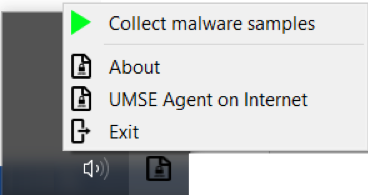
\includegraphics[width=0.4\textwidth]{./figures/UMSEAgent}
\end{figure}

\subsection{UMSE server}

The UMSE server is composed of the following files (see
Figure~\ref{fig:UMSEServer}):
\begin{figure}
  \centering
  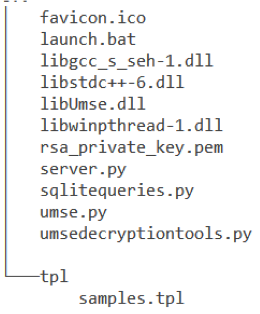
\includegraphics[width=0.4\textwidth]{./figures/UMSEServer}
  \caption{\label{fig:UMSEServer} Structure of the UMSE server.}
\end{figure}

\begin{itemize}
\item \texttt{favicon.ico}: The web application favicon.
\item \texttt{launch.bat}: Simple batch file to start the program.
\item \texttt{libgcc\_s\_sheh-1.dll}, \texttt{libstdc++-6.dll},
  \texttt{libwinpthread-1.dll}: Some \texttt{libUmse.dll} dependencies.
\item \texttt{libUmse.dll}: The compiled UMSE C/C++ library.
\item \texttt{rsa\_private\_key.pem}: RSA Private key which allows UMSE sample
  parts decryption.
\item \texttt{server.py}: A Cherrypy server implementing an extremely simple
  intelligence webpage and REST API to allow the agent to operate with
  samples. Samples are stored in a SQLite database.
\item \texttt{sqlitequeries.py}: SQLite queries are defined here.
\item \texttt{umse.py}: Kaitai Struct UMSE file format parser.
\item \texttt{umsedecryptiontools.py}: Python functions allowing to decrypt an
  UMSE entry (functionality is implemented by \texttt{libUmse.dll}. It is only
  a bridge to it).
\item \texttt{tpl/samples.tpl}: HTML with JAVASCRIPT template used by
  Cherrypy.
\end{itemize}

This is how intelligence panel looks like. It is extremely simple. Only
sample listing (- and + are shortcut keys to go back and forward), sample
search, and sample downloading features are implemented. But note that REST
API requires authentication in order to decrypt samples, and every decryption
operation is logged into SQLite database access logging table.
\begin{figure}[h]
  \centering
  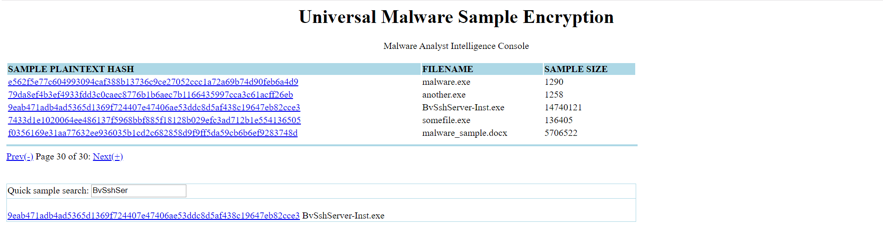
\includegraphics[width=0.99\textwidth]{./figures/UMSEPanel}
  \caption{\label{fig:UMSEPanel} Some caption.}
\end{figure}

\subsection{UMSE Shell}

An extremely simple command line tool implemented in Python which allows you
to interact with the UMSE server. All implementation remains into the
\texttt{umse\_shell.py} file which looks as follows:
\begin{figure}[h]
  \centering
  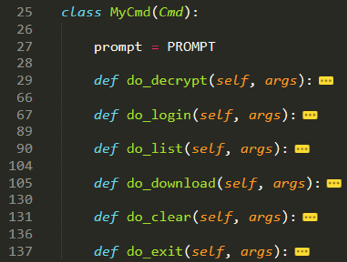
\includegraphics[width=0.4\textwidth]{./figures/UMSEShell}
\end{figure}

\begin{table}[h]
  \centering
  \begin{tabular}{|l|p{0.7\textwidth}|} \hline
    \textsc{Method} & \textsc{Description} \\ \hline
    \texttt{do\_list} &	List samples stored in the UMSE server. \\ \hline
    \texttt{do\_download} & Download samples from the server. \\ \hline
    \texttt{do\_login} & Login into the server. \\ \hline
    \texttt{do\_decrypt} & Decrypt an entry of an UMSE sample (login is
                           required). \\ \hline
    \texttt{do\_clear} & Clear screen. \\ \hline
    \texttt{do\_exit} & Exit the program. \\ \hline
  \end{tabular}
\end{table}

And this is how this console looks like.
\begin{figure}[h]
  \centering
  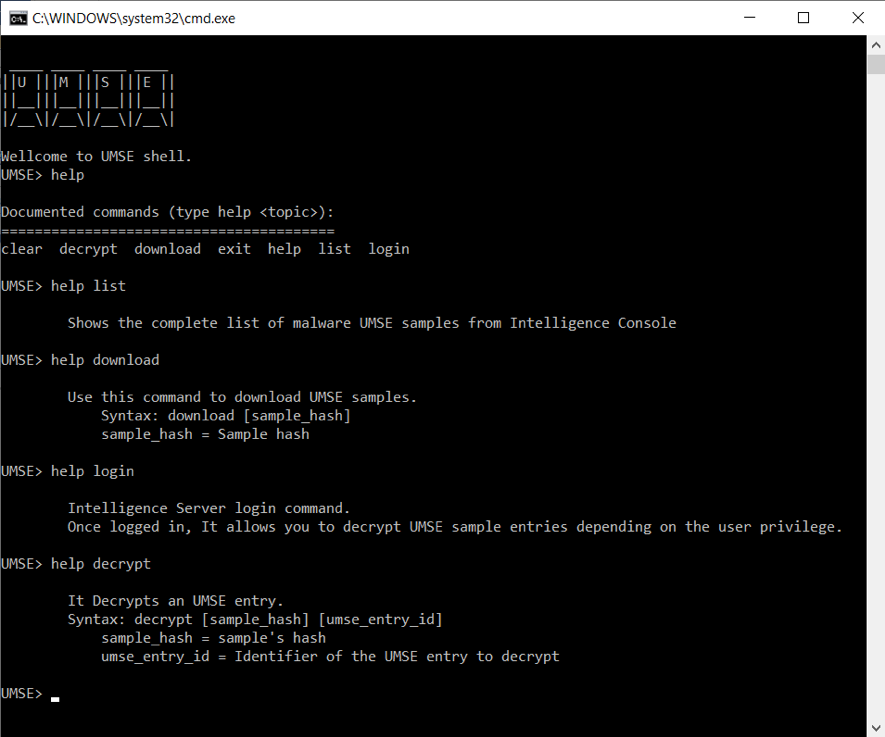
\includegraphics[width=0.95\textwidth]{./figures/UMSEConsole}
\end{figure}

\subsection{UMSE tools}

The UMSE format RSA encryption is a key feature but, in some situations like
when sharing malware between colleagues encryption can be a hindrance. In this
situations you can embed the RSA private key into the sample and don’t care
about encryption anyway.  In this way, the analyst is benefiting himself by
using a specific format to share malware files and, in a future version of
this simple python tool, of metadata and heterogeneous element per sample
appending capabilities of UMSE format.  You can use a simple Python tool
(\texttt{tool\_for\_single\_users.py}) developed for this purpose:
\begin{figure}[h]
  \centering
  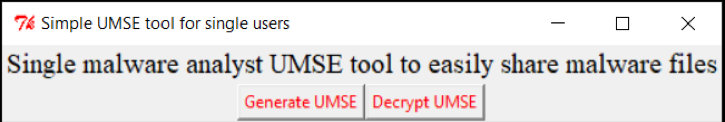
\includegraphics[width=0.75\textwidth]{./figures/UMSETool}
\end{figure}